\documentclass{article}

% if you need to pass options to natbib, use, e.g.:
% \PassOptionsToPackage{numbers, compress}{natbib}
% before loading nips_2017
%
% to avoid loading the natbib package, add option nonatbib:
%\usepackage[nonatbib]{nips_2017}

% \usepackage{nips_2017}

% to compile a camera-ready version, add the [final] option, e.g.:
\usepackage[final]{nips_2017}

\usepackage[utf8]{inputenc} % allow utf-8 input
\usepackage[T1]{fontenc}    % use 8-bit T1 fonts
\usepackage{hyperref}       % hyperlinks
\usepackage{url}            % simple URL typesetting
\usepackage{booktabs}       % professional-quality tables
\usepackage{amsfonts}       % blackboard math symbols
\usepackage{nicefrac}       % compact symbols for 1/2, etc.
\usepackage{microtype}      % microtypography
\usepackage{graphicx}
\graphicspath{{./images/}}


% Additional
\usepackage{natbib}
% Additional
\usepackage{amsmath, amssymb}
\usepackage{bm}
\usepackage{tabularx}
\usepackage{booktabs}
\usepackage{caption, subcaption}
\usepackage{multirow}

\title{Spark Project Report 1}

% The \author macro works with any number of authors. There are two
% commands used to separate the names and addresses of multiple
% authors: \And and \AND.
%
% Using \And between authors leaves it to LaTeX to determine where to
% break the lines. Using \AND forces a line break at that point. So,
% if LaTeX puts 3 of 4 authors names on the first line, and the last
% on the second line, try using \AND instead of \And before the third
% author name.

\author{
  Shun Zhang \\
  School of Data Science\\
  Fudan University\\
  Shanghai, China \\
  \texttt{15300180012@fudan.edu.cn} \\
}

\begin{document}
% \nipsfinalcopy is no longer used

\maketitle

\section{E Problems}

\subsection{Problem E1}
\paragraph{analysis}
Here our goal is to find the oldest man within the records available. This problem can be divided into two sub-problems:
\begin{itemize}
\item find all the MAN
\item find the oldest one
\end{itemize}
and their relating solutions in pySpark requires no shuffle dependency. The \emph{order key} is to find the one with the earliest birth date, where we find \[old = argmin_{record}\{ 1000*year + 50*month + day \}\]

\paragraph{result}
There are a few records, of which the date of birth is censored, such as `//1932'. As for these censored record, we fill them based on the `as latest as possible' rule. For example, `//1932' is filled as '31/12/1932', `2/3/' is filled as '2/3/2018'. By doing this, we have a greater chance to find the oldest man.

Finally, we find the target record as follows:

\emph{33475111 24422710170 MEHMET ALI CEVIK AYYUS MEHMET E OGUZELI //1330 KILIS ELBEYLI KILIS ELBEYLI DOGAN MAH. GUL SOKAK 7 <NULL>}

\textbf{Note that} the man we found is about 700 years old if he is still alive, which is impossible as far as I know. However, here we have no idea about whether a citizen is alive or not. So, we just treat them all as alive.


\subsection{Problem E2}
\paragraph{analysis}
Here, our goal is to find the most popular letters in one's NAME. This problem can be divided into two sub-problems:
\begin{itemize}
\item split every name into letters (flatmap)
\item count every letter and put them in order
\end{itemize}
and we only need one shuffle dependency: \emph{reduceByKey}.

\paragraph{result}
Note that here we treat NAME as both first name and last name. Also, we treat `most popular' as top-3. The results are:
\begin{table}[ht]
\centering
\begin{tabular}{lccc}
\toprule
Letter & A & E & I \\
\midrule
Frequency & 57623513 & 39619607 & 34493003 \\
\bottomrule
\end{tabular}
% [(u'A', 57623513), (u'E', 39619607), (u'I', 34493003), (u'N', 26440665), (u'R', 24978398), (u'U', 24072703), (u'L', 22802085), (u'M', 20796307), (u'S', 20375160), (u'K', 19204812)]
\end{table}


\subsection{Problem E3}
\paragraph{analysis}
Here our goal is to find the number of people in a certain range of age. This problem is quite similar to problem E2.

\paragraph{result}
An interesting phenomenon is that there is no people under 18 in this dataset. The results are:
\begin{table}[ht]
\centering
\begin{tabular}{lccccc}
\toprule
Age & 0-18 & 19-28 & 29-38 & 49-55 & >60 \\
\midrule
Frequency & 0 & 1130969 & 8881641 & 4694314 & 9555000 \\
\bottomrule
\end{tabular}
% [('49-55', 4694314), ('60-', 9555000), ('others', 10465669), ('19-28', 1130969), ('29-38', 8881641)]
\end{table}
Here we only need one shuffle dependency: \emph{reduceByKey} and also there are other people who age in range 39-48 or 56-60, of which the frequency is 10465669.

\subsection{Problem E4}
\paragraph{analysis}
Here our goal is to find the number of people born in a certain month. This problem is quite similar to problem E3. Also we only need one shuffle dependency: \emph{reduceByKey}.

\paragraph{result}
There are one record with birth month `14', one record with month `15' and 461 records with month `0'. Also, there are 43050 records, whose birth month is censored. These records are all treated as invalid data. The results of the valid records are:
\begin{figure}[ht]
\centering
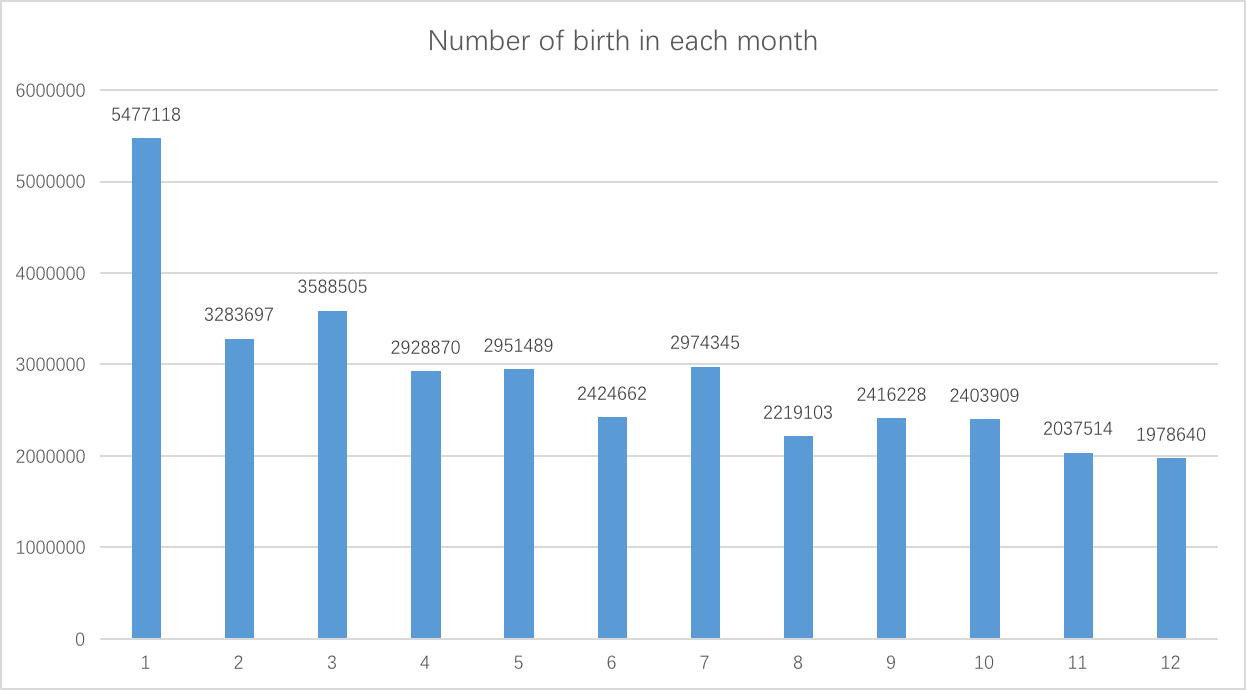
\includegraphics[width=0.7\linewidth]{E4}
\end{figure}
% [(u'4', 2928870), (u'14', 1), (u'3', 3588505), (u'9', 2416228), (u'2', 3283697), (u'1', 5477118), (u'8', 2219103), (u'0', 461), (u'7', 2974345), ('censored', 43050), (u'6', 2424662), (u'5', 2951489), (u'11', 2037514), (u'10', 2403909), (u'12', 1978640), (u'15', 1)]


\subsection{Problem E5}
\paragraph{analysis}
Here our goal is to find the number of males and females respectively and then derive the male-female ratio. The only shuffle dependency here is: \emph{reduceByKey}.

\paragraph{result}
The result is shown in Figure~\ref{fig-mf} and the male-female ratio is about $1:1.0222$.
\begin{figure}[ht]
\centering
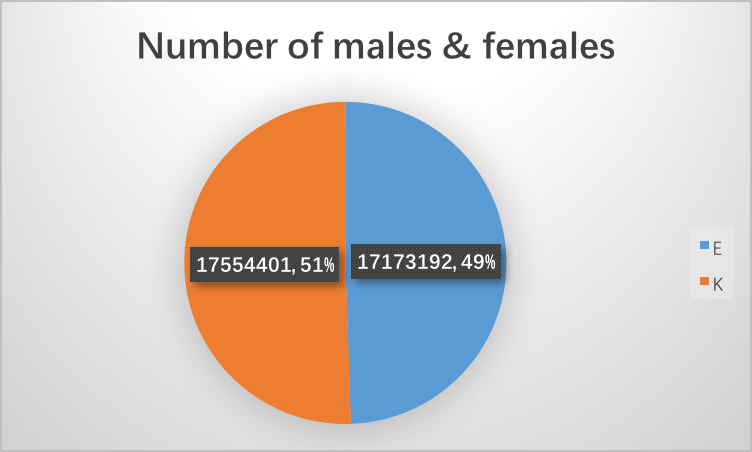
\includegraphics[width=0.5\linewidth]{E5}
\caption{Total number of the males and females}
\label{fig-mf}
\end{figure}
% [(u'E', 17173192), (u'K', 17554401)]    


\section{N Problems}


\subsection{Problem N1}
\paragraph{analysis}
Here our goal is to find the top-10 last name of males and females respectively. This problem is quite similar to problem E2.
\paragraph{result}
It is interesting that the results for male and female are quite similar. And the only shuffle dependency is: \emph{reduceByKey}.
\begin{itemize}
\item Male
\begin{figure}[ht]
\centering
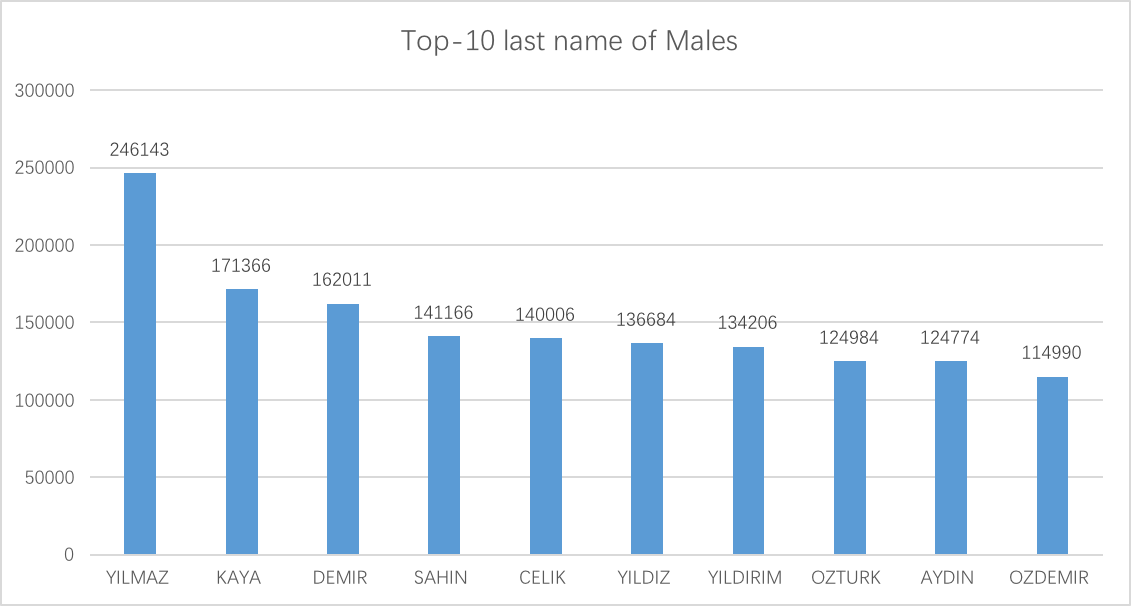
\includegraphics[width=0.7\linewidth]{N1_1}
\end{figure}
% [(u'YILMAZ', 246143), (u'KAYA', 171366), (u'DEMIR', 162011), (u'SAHIN', 141166), (u'CELIK', 140006), (u'YILDIZ', 136684), (u'YILDIRIM', 134206), (u'OZTURK', 124984), (u'AYDIN', 124774), (u'OZDEMIR', 114990)]
\item Female
\begin{figure}[ht]
\centering
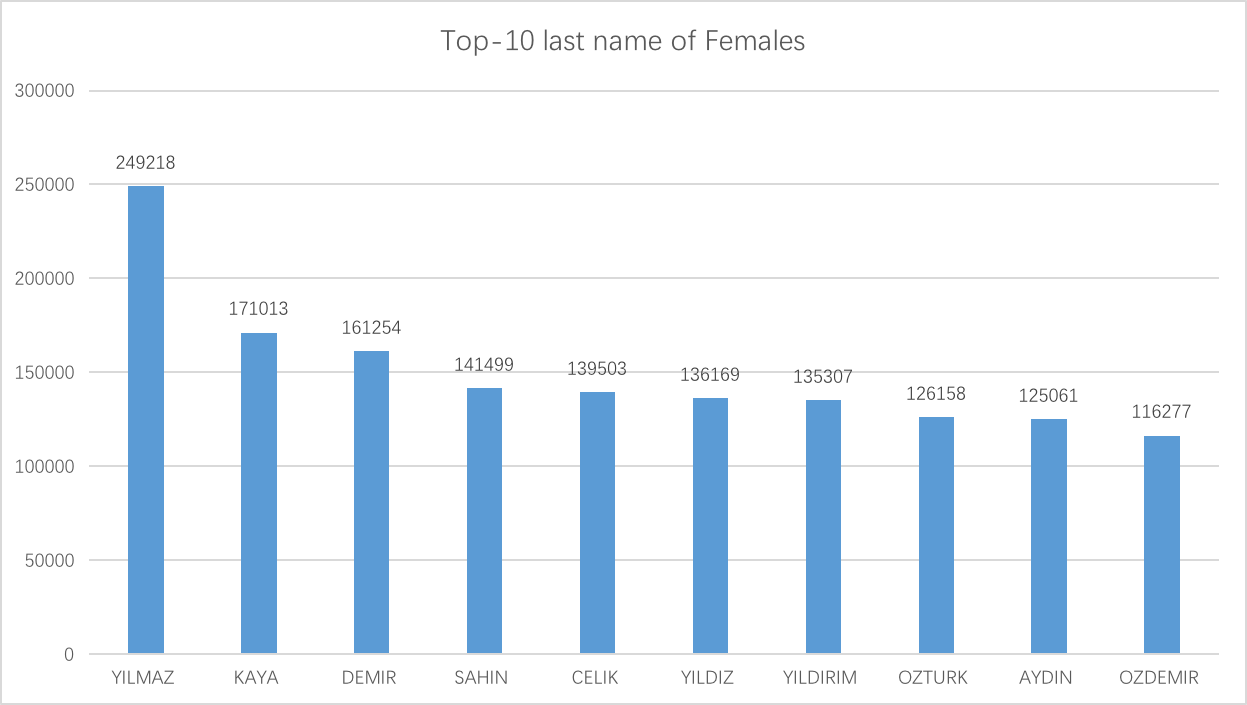
\includegraphics[width=0.7\linewidth]{N1_2}
\end{figure}
% [(u'YILMAZ', 249218), (u'KAYA', 171013), (u'DEMIR', 161254), (u'SAHIN', 141499), (u'CELIK', 139503), (u'YILDIZ', 136169), (u'YILDIRIM', 135307), (u'OZTURK', 126158), (u'AYDIN', 125061), (u'OZDEMIR', 116277)]
\end{itemize}



\subsection{Problem N2}
\paragraph{analysis}
Here, our goal is to find the average age of each city. This job can be divided into two steps:
\begin{itemize}
\item get the sum of ages of a certain city's citizens
\item get the total number of the citizens above
\end{itemize}
The two steps can be integrated into a triad: (city, sum of age, total number), which can be derived by `reduceByKey' in PySpark.
\paragraph{result}
The results are shown in an ascending order in Figure~\ref{fig-1} and the only shuffle dependency is: \emph{reduceByKey}.
\begin{figure}[ht]
\centering
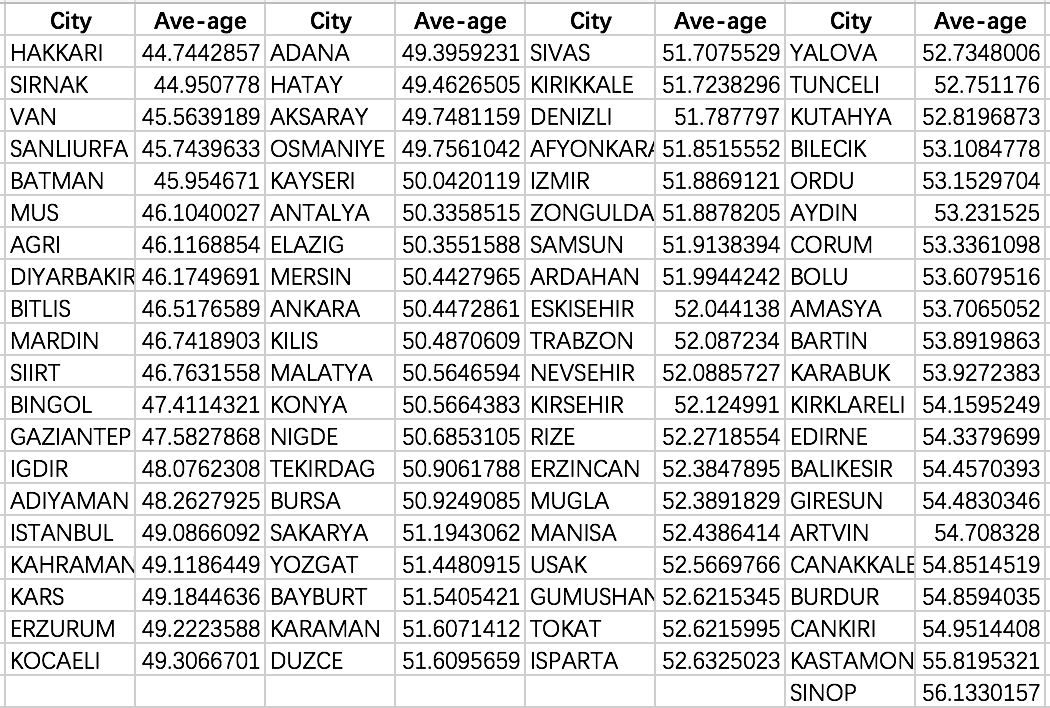
\includegraphics[width=0.7\linewidth]{N2}
\caption{Average age of each city.}
\label{fig-1}
\end{figure}

\subsection{Problem N3}
\paragraph{analysis}
Here our goal is to find the top-5 cities with low average age. And the only shuffle dependency is: \emph{reduceByKey}.
\paragraph{result}
The result can be easily derived from Figure~\ref{fig-1}, which is \emph{HAKKARI, SIRNAK, VAN, SANLIURFA and BATMAN}.

\subsection{Problem N4}
\paragraph{analysis}
Here our goal is to find the top-3 popular last name in the top-10 cities in population. My solution is quite simple that
\begin{enumerate}
\item find the top-10 cities in population
\item find the top-3 popular last name for each city
\end{enumerate}
which requires two shuffle dependencies: \emph{reduceByKey} and \emph{groupByKey}.

\paragraph{result}
The results are shown in Table~\ref{table-1}.
\begin{table}[ht]
\centering
\caption{ Top-3 popular last name in the top-10 cities in population}
\label{table-1}
\begin{tabular}{llll}
\toprule
City & Last Name 1(Num) &  Last Name 2(Num) &  Last Name 3(Num) \\
\midrule
ISTANBUL & YILMAZ(97328) & KAYA(61306) & DEMIR(54817) \\
ANKARA & YILMAZ(33694) & SAHIN(22316) & OZTURK(19988) \\
IZMIR & YILMAZ(23224) & KAYA(15718) & DEMIR(13515) \\
BURSA & YILMAZ(19199) & AYDIN(13771) & OZTURK(12118) \\
AYDIN & YILMAZ(10441) & KAYA(8274) & DEMIR(7948) \\
ADANA & YILMAZ(11196) & KAYA(9225) & DEMIR(8046) \\
KONYA & YILMAZ(9966) & CELIK(7150) & KAYA(6808) \\
ANTALYA & YILMAZ(14686) & KAYA(8802) & CELIK(8432) \\
MERSIN & YILMAZ(10995) & SAHIN(8196) & KAYA(7273) \\
KOCAELI & YILMAZ(11744) & AYDIN(6876) & KAYA(6736) \\
\bottomrule
\end{tabular}
\end{table}


\subsection{Problem N5}
\paragraph{analysis}
Here our goal is to find the top-2 popular birth month in the top-10 cities in population. This problem is quite similar to problem N4, which requires two shuffle dependencies: \emph{reduceByKey} and \emph{groupByKey}.

\paragraph{result}
The results are shown in Table~\ref{table-2}.
\begin{table}[ht]
\centering
\caption{ Top-2 popular birth month in the top-10 cities in population}
\label{table-2}
\begin{tabular}{lll}
\toprule
City & Birth month 1(Num) & Birth month 2(Num) \\
\midrule
ISTANBUL & Jan.(860655) & Mar.(618980)  \\
ANKARA & Jan.(317030) & Mar.(222616)  \\
IZMIR & Jan.(268901) & Mar.(197023)  \\
BURSA & Jan.(171561) & Mar.(124556)  \\
AYDIN & Jan.(135393) & Mar.(100959)  \\
ADANA & Jan.(193277) & Mar.(94205)  \\
KONYA & Jan.(143228) & Mar.(96847)  \\
ANTALYA & Jan.(145205) & Mar.(94399)  \\
MERSIN & Jan.(132807) & Mar.(77870)  \\
KOCAELI & Jan.(96775) & Mar.(73050)  \\
\bottomrule
\end{tabular}
\end{table}
An interesting thing is that the top-2 popular birth months are the same among these ten cities.




%\clearpage
% Bibliography
%\bibliography{biblio}
%\bibliographystyle{plainnat}

\end{document}
